% This is the template for submission of abstracts to NetSci 2024 in Québec, Canada.
% It is modified from NetSci2017, which was inspired by that of NetSci2016 and that of STATPHSY25.
% The editor of the booklet reserves the right to modify your submission.

% To process this file run LaTeX2e

% ******** DO NOT EDIT ****************
\documentclass[10pt]{article}
% \usepackage{mathptmx}
\usepackage[letterpaper,margin=20mm]{geometry}
\usepackage{graphicx}
\usepackage{lmodern}
\renewcommand{\familydefault}{\sfdefault}
\pagestyle{empty}
\setlength{\parskip}{0.25\baselineskip}
\renewcommand{\title}[1]{{\noindent\large\bfseries#1\medskip\\}}
\renewcommand{\author}[2]{{\noindent #1 \medskip\\ \noindent \small #2 \medskip\\}}
% *************************************

\begin{document}

% ********** USER DEFINED *************


% Enter title here
\title{A Regional Spatial Graph Convolutional Neural Network (RSGCN) for Spatially Embedded Network Modeling}
\author{
    % Enter author(s) here
    Xudong Fan\textsuperscript{1}
    and
    Jürgen Hackl,\textsuperscript{1}
}
{
    % Enter affiliation(s) here
    1. Princeton University, Princeton, NJ, USA\\
}



% Enter abstract here. Please keep everything within one page.

The functional behaviors of large-scale systems can often be interpreted as complex networks. However, such complex networks are often difficult to observe directly in the real world [1]. For example, social networks and social influence are difficult to obtain despite the wide availability of online data [2]. The networks of epidemic transmission are also difficult to observe directly [3]. Although previous studies have employed a wide range of graph theories for network modeling, the spatial aspects of these graphs are often overlooked. Many real-world systems, such as transportation infrastructure and biological systems, are influenced by spatial and physical constraints[4]. Only recently have researchers begun to explore the modeling of complex networks while considering their spatial information [5].

To model such spatially embedded networks, this study proposed a regional spatial graph convolutional network (RSGCN) for network connection prediction. Unlike traditional graph theory-based models which assume the graphs are independent of the space, the proposed method is developed for systems that are embedded in a spatial space. The spatial information of the systems has been considered in the network modeling process and thereby achieved a higher model accuracy. To test and evaluate the performance of the proposed model, three graph datasets were used for training and validating purposes, including a synthetic graph dataset, a real-world road network, and a real-world river network. The modeling results of RSGCN were then compared to those of two other geometric deep learning models, GraphSAGE and Spatial Graph Convolutional Network (SGCN).

Our results indicate that the proposed RSGCN outperformed the weakest model by 6.65\%, 37\%, and 59\%, respectively, regarding the F1 score in all three network datasets. The proposed model also predicted a more accurate edge length distribution, node degree distribution, and number of component distribution, compared to the other models. The proposed method is the first variant of graph convolutional networks (GCNs) that can consider regional spatial information. It is also the first time using a geometric deep learning model for spatially embedded network modeling.


\bigskip
{\small
    \noindent[1] Peixoto and Tiago P. (2019) {Network {{Reconstruction}} and {{Community Detection}} from {{Dynamics}}}, {Physical Review Letters} \\
    \noindent[2] {Bakshy, Eytan and Rosenn, Itamar and Marlow, Cameron and Adamic, Lada} (2012), {The Role of Social Networks in Information Diffusion}, {Proceedings of the 21st International Conference on {{World Wide Web}}}\\
    \noindent[3] {Keeling, Matt J. and Rohani, Pejman}(2002),{Estimating Spatial Coupling in Epidemiological Systems: A Mechanistic Approach},{Ecology Letters}\\
    \noindent[4] {Barnett, L. and Di Paolo, E. and Bullock, S.} (2007), {Spatially Embedded Random Networks},{Physical Review E}\\
    \noindent[5] {Hackl, J{\"u}rgen and Adey, Bryan T}(2019), {Modelling Multi-Layer Spatially Embedded Random Networks}, {Journal of Complex Networks}\\
}


\begin{figure}[!h]
    \centering
    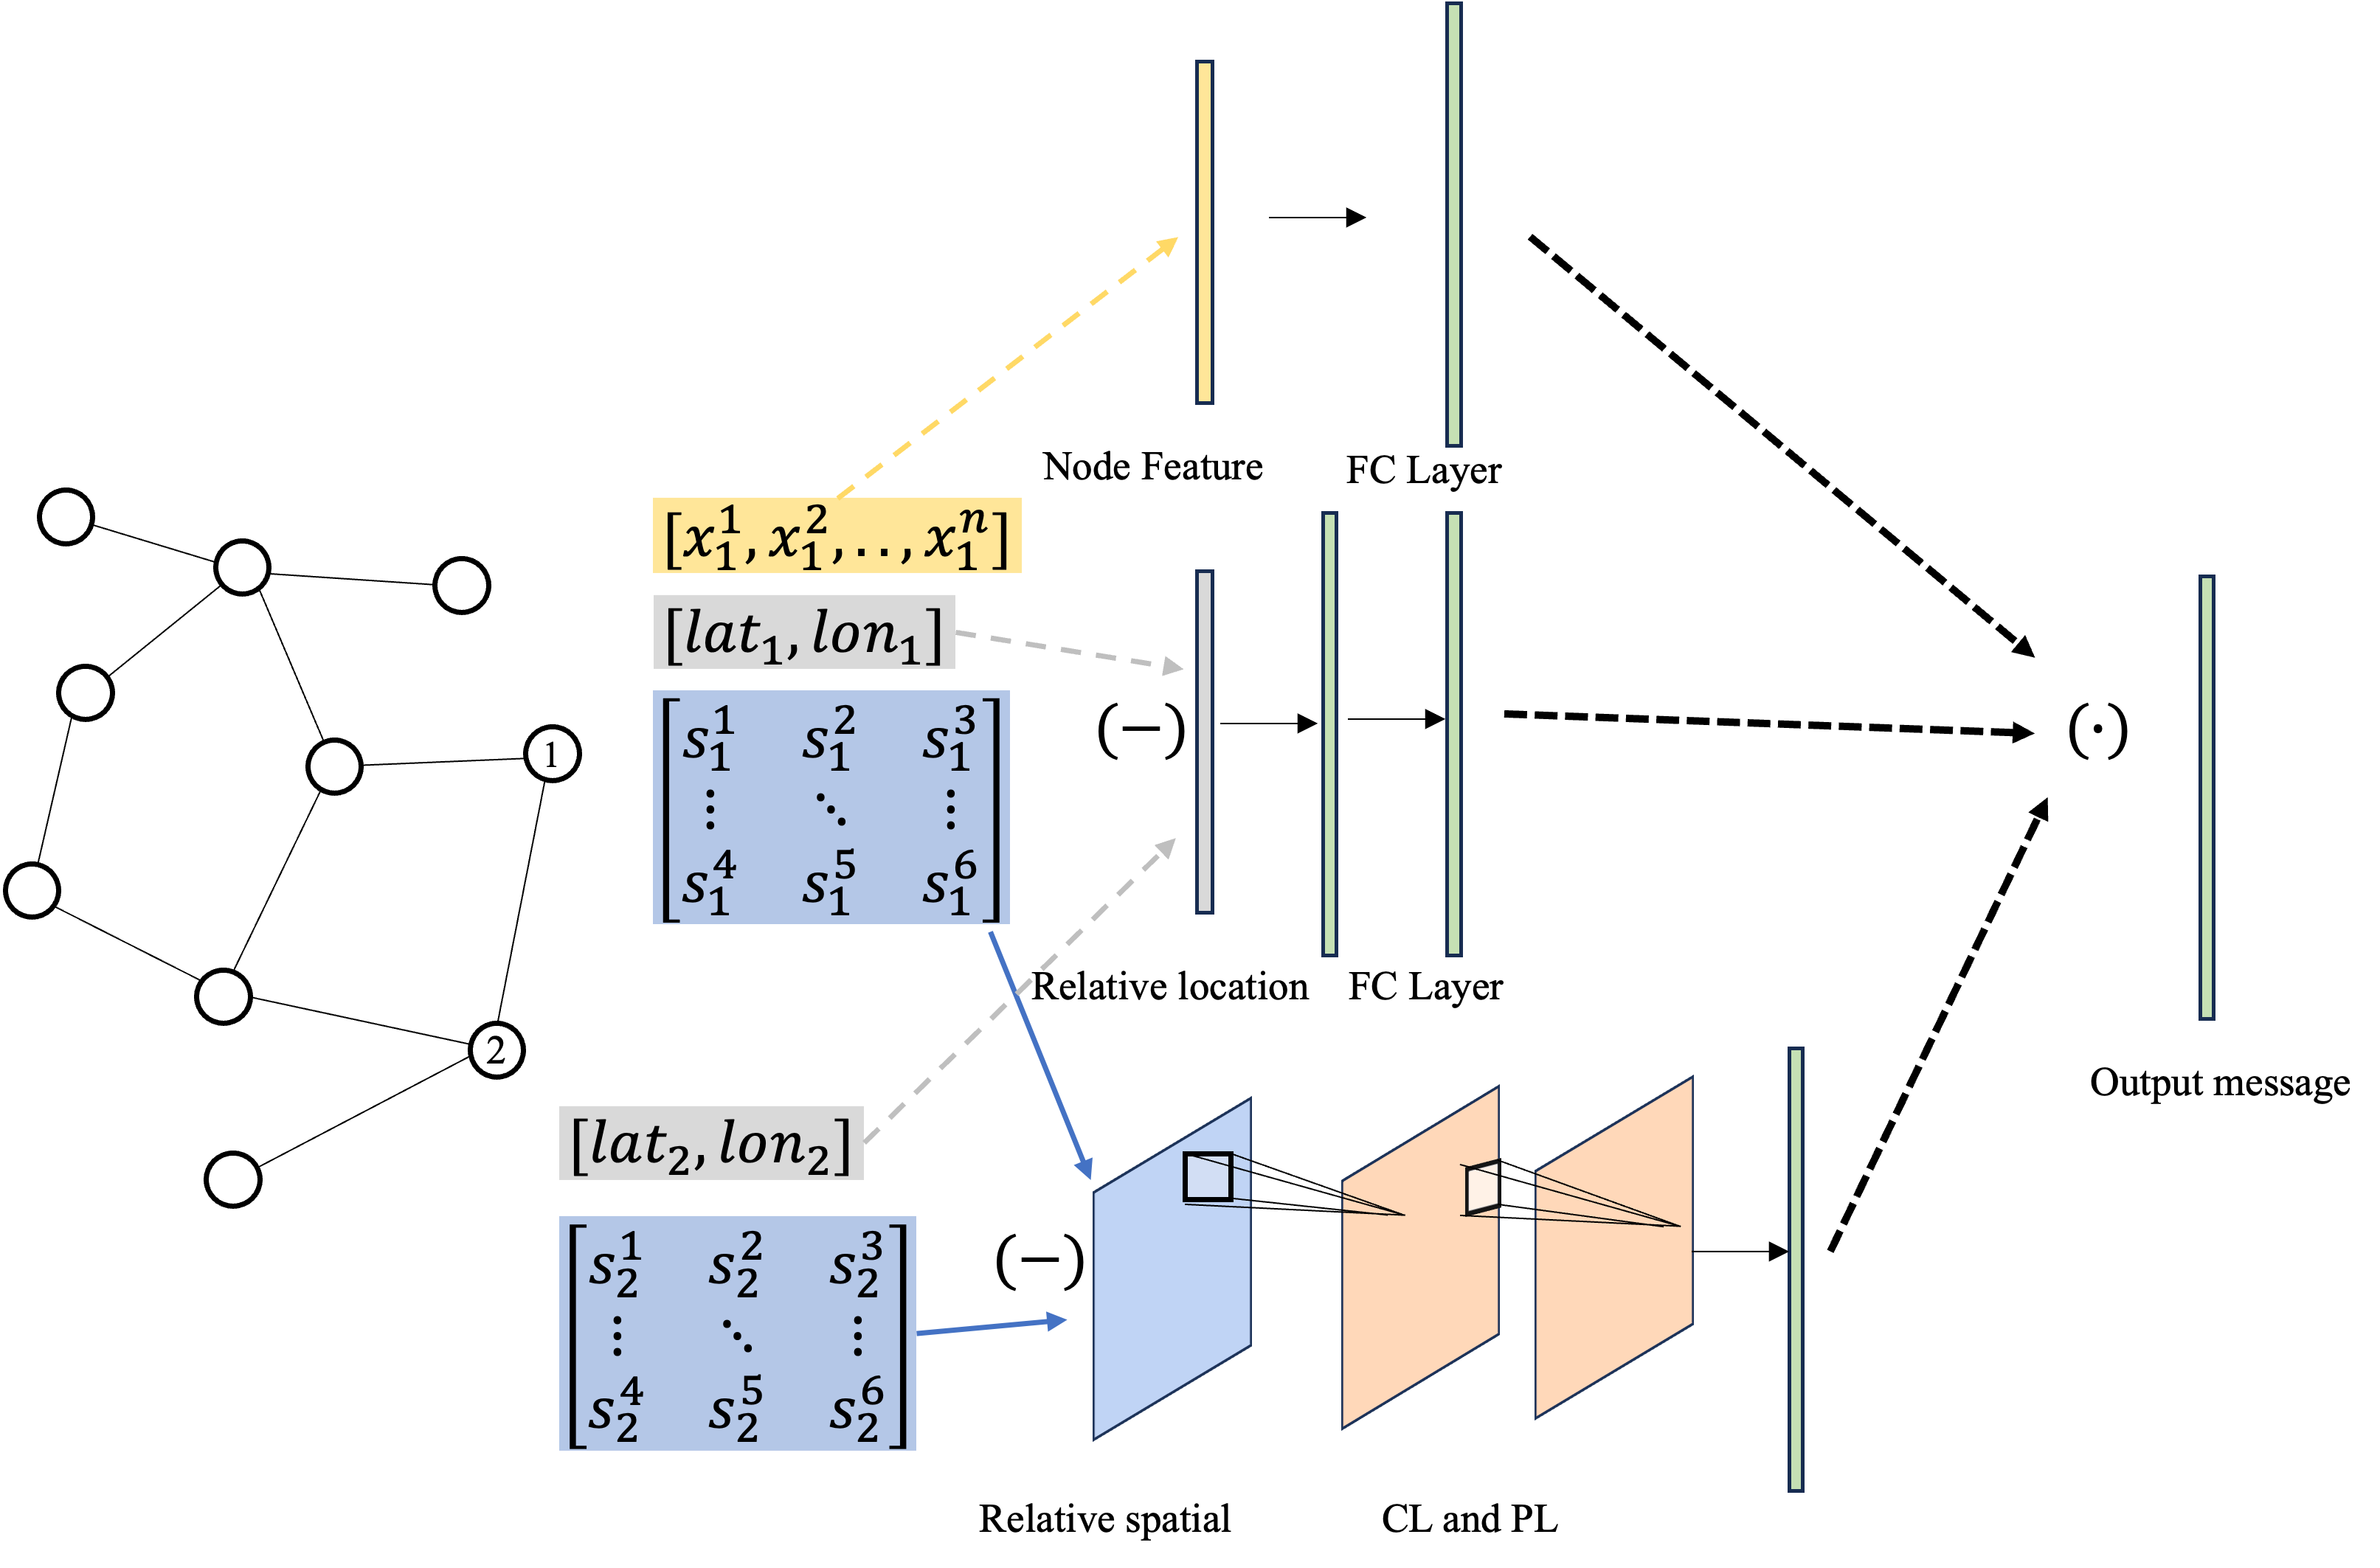
\includegraphics[width=0.5\textwidth]{RSGCN.png}
    \caption{The Proposed RSGCN Architecture}
\end{figure}


% *************************************
\end{document}